\chapter[Weak Coupling of Meta-Materials for FD-FT THz EPR]{Weak Coupling of Meta-Materials with Ensemble of Electron Spins: Surface EPR Signal Enhancement in the THz Bandgap.}
\chaptermark{FD-FT THz EPR with Meta-Materials}


As the microwave frequency is increased, single-mode cavity resonators and samples become geometrically small. At even higher frequencies, the further reduced dimensions prevent the fabrication of conventional resonators due to technical limitations. In order to increase sensitivity at higher frequencies the use of non-resonant structures, such as the so-called ``bucket'' sample holder, can be employed. In these non-resonant structures the sample volume is increased to fill the bucket which provides a large filling factor $\eta$ with a Q$_0$-value effectively at unity. \cite{grinbergVHF} However, the shape of the bucket resonator is adapted to powders or solutions filled in tubes, and is not optimal for studies of thin films or surfaces. The ability to measure thin films is crucial for the study of a variety of interesting samples, such as thin magnetic films, thin-film electronic devices, solar cells or other 2D paramagnetic samples.

The transition from volume samples, such as those in single-mode cavity resonators, to planar samples requires a concentration of the magnetic component of the time-varying excitation field on a cross-sectional area. For example, the plane-concave Fabry-P\'{e}rot resonator, which comprises of a resonant structure with one concave mirror and one flat mirror, forms a standing-wave pattern with a maximum magnetic field on the flat-mirror surface. \cite{grinbergVHF} Plane-concave Fabry-P\'{e}rot resonators exhibit very high Q-values and, due to the simplified geometry, can be designed to operate at frequencies higher than 200~GHz. \cite{Clarke1982Fabry, BraakmanFabry} However, the resonator geometry still scales with frequency and, due to the standing-waves within the resonator, the filling factor can be quite low for thin films. In order to maximize the EPR signal intensity for thin film samples, we seek a resonant geometry where the cross-sectional sample area is not dependent on the operating frequency and the filling factor is maximized. 

One solution is to create a series of single nano-resonators that can be placed in periodic sequences to form a large two-dimensional array. Despite the periodic nano-structure, the incident excitation wave interacts with the surface as a bulk material. \cite{Yen04} This bulk material, called a meta-material, can be characterized by the single and periodic geometry, mutual coupling between elements, eigenfrequency, and $Q_0$-value. Meta-material characteristics can then be used to determine the frequency dependent properties. The frequency dependent properties of meta-materials were theoretically proposed in 1968 as materials with bulk properties that mimic frequency dependent negative electric-permittivity $\epsilon_r(\omega)$ and magnetic permeability $\mu_r(\omega)$. \cite{Veselago68} The ability to tune these properties allows a negative refraction index to be designed for perfect lensing, i.e. images with better resolution than the diffraction limit. \cite{Smith04} Unlike single-mode cavities that require the sample to be placed on an axis of maximum sensitivity, meta-materials can provide a bulk material-like enhancement of a sample at a surface.

Recently, it was found that the split-ring resonator (SRR) geometry at sub-wavelength dimensions can be placed in a periodic fashion on a surface and behave as a meta-material over a broad frequency range. \cite{Smith00,Yen04,Linden04} This first realization was shown for the low GHz range, \cite{Smith00} then for around 1~THz, \cite{Yen04} and for 100~THz. \cite{Linden04} The negative $\mu_r(\omega)$ leads to a resonance effect in the non-magnetic meta-material. Interestingly, meta-material surfaces operating in the THz region have been employed for ultra-sensitive bio-sensing due to their ability to sense small dielectric changes on a surface. \cite{C7NR03824K} For a bio-sensing experiment, THz frequency microwave fields are incident on the meta-material and the resulting transmission is monitored for changes as bio-material passes the resonant geometry. \cite{Lee2017}

\begin{figure}[htpb]
\centering
  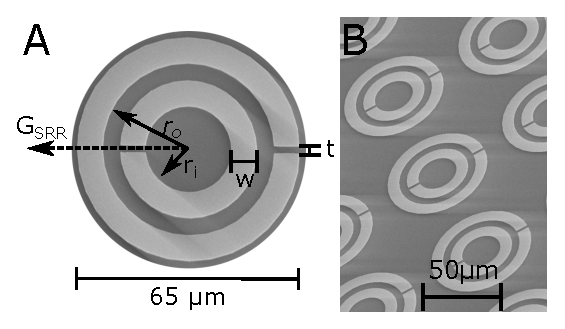
\includegraphics{Kapitel/Ch3-Images/01-Measurements.eps}%
  \caption[Microscope image of the SRR geometry.]{ A) Microscope image of the fabricated profile of the dual-ring split-ring resonator (SRR) on quartz glass. In this work dimensions are as follows: r$_o$ is 25~$\mu$m, r$_i$ is 12.5~$\mu$m, w is 7.5~$\mu$m , and t is 2~$\mu$m. The vector parallel to the gap is illustrated G$_{SRR}$. B) To create a meta-metallic surface each SRR element is spaced 80~$\mu$m apart from center-to-center.}
  \label{ch3-fig:sizes}
\end{figure}

Herein, we present the characterization and experimental realization of a meta-material by a split-ring resonator array (SRRs) for the use of detecting EPR transitions in the 100~GHz to 1~THz frequency range (3.336-33.356~cm$^{-1}$; THz-bandgap). The SRRs have an operating frequency of approximately 420~GHz (14~cm$^{-1}$; free-space wavelength $\lambda$ of 713.79~$\mu$m). A single SRR outer diameter is 65~$\mu$m, geometry shown in Fig.~\ref{ch3-fig:sizes}A. Therefore each SRR is less than 1/10th of a wavelength, and is spaced 80~$\mu$m from the next resonator in a periodic fashion creating the bulk-material. The SRRS, shown in Fig.~\ref{ch3-fig:sizes}B, were placed on a quartz substrate that has an overall diameter of 12~mm providing very large surface area for an operating frequency of 420~GHz.

The results were duplicated with a lumped-circuit transmission\-/line analytic model. The lumped-circuit transmission\-/line model, unlike current literature, takes into account both inductive and capacitive coupling. This distinction is important when the interaction of magnetic resonance coincides with the resonant frequency of the SRRs.

The validity of the analytical model was established and used to further understand the interactions that arise between the meta-material and the electron-spins ensemble. Furthermore, the analytical model was used to define the system in terms of weak- and strong-coupling. Through this new understanding, we illustrate the potential of meta-material arrays for resonant EPR detection at very high frequencies for thin film samples. 

\section{Methods}
In order to characterize the SRRs we employ Frequency-Domain Fourier-Transform THz-EPR (FD-FT THz EPR) experiments. FD-FT EPR is a method to detect magnetic transitions in the THz-bandgap using a interferometer and bolometer detector. \cite{Schnegg09,NEHRKORN201710} Such methods allow for broad-band detection of EPR in the frequency domain while stepping the static magnetic field through the EPR resonance condition. Over the last decade, several other EPR instruments were built which operate at microwave frequencies in the THz-bandgap. \cite{Disselhorst95, Hassan00, vanTol05, Zvyagin09, Takahashi09, C7CP07443C, Lu2017} The SRRs were characterized and coupled to the electron-spin ensemble of a thin film of the high-spin Fe-ion cluster hemin. The high-spin Fe EPR signal was collected by following the feature located at the effective $g=6$ position which passes through the frequency of the split-ring resonator as the magnetic field is increased. 

Coherent broadband excitation profiles are required FD-FT EPR experiments. However, at such frequencies, excitation power is limited (mW range) and the frequency range of such sources is limited making frequency domain experiments rather impractical. To overcome these limitations, an alternative excitation and detection scheme has been developed for FD-FT EPR to be performed using a high-power broad-band source, such as a coherent beam-line from the BESSY II synchrotron (Helmholtz-Zentrum Berlin; Berlin, DE). From this setup the EPR spectrum can be ascertained with good signal-to-noise ratio making FD-FT EPR a powerful technique to obtain accurate zero-field splitting parameters. \cite{Nehrkorn13,Nehrkorn15,NEHRKORN201710}

\begin{figure}[htpb]
\centering
  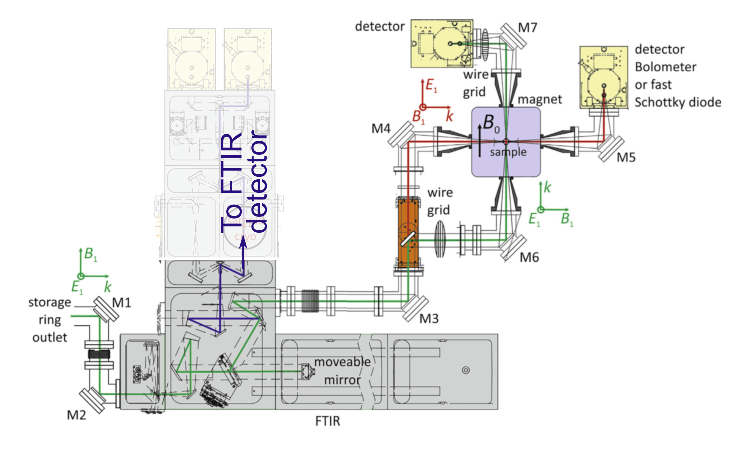
\includegraphics{Kapitel/Ch4-Images/Ch4-ExperimentSetup.eps}%
  \caption[Schematic Overview of FT-FD THz-EPR setup.]{Shown is the schematic overview of the FT-FD THz-EPR setup. The incident wave from the storage ring is sent through a series of mirrors (M1-M3) as it is guided through an FTIR interferometer setup (green line). Here, the wave can be rotated (M4) and sent through the static magnetic field (\textbf{B}$_0$) to M5 and a bolometer detectir (red line) or reflected directly (M6) through the static magnetic field (\textbf{B}$_0$) to M7 and a bolometer detector (green line). An alternative path allows FTIR to be performed (blue line).}
  \label{ch4-fig:ExFDFTSetup}
\end{figure}

Frequency-Domain Fourier-Transform THz-EPR experiments in this work were conducted at the synchrotron BESSY II. The experimental setup is shown in Fig.~\ref{ch4-fig:ExFDFTSetup} \cite{Schnegg09,Nehrkorn13,NEHRKORN201710} In short, intense and coherent broadband linearly-polarized radiation in the THz-gap is provided by the synchrotron BESSY II from the storage ring. \cite{AboBakr02} After passing through the interferometer of an FTIR spectrometer (moveable mirror), linearly-polarized THz radiation passes a roof top mirror which allows rotation of the THz TEM-wave polarization to any direction perpendicular to the direction of propagation $\vect{k}$, depicted as the green or red path. Next, the THz radiation is guided through a super-conducting magnet (Oxford Spectromag, $\pm$11~T maximal field). The sample is inserted in a variable temperature inset (2-300~K) inside the magnet. Finally, the THz radiation is detected with a highly sensitive Si bolometer immersed in a pumped liquid-Helium bath (1.3~K). In this work, the experimental resolution was set to 0.2~cm$^{-1}$ (max resolution: 0.0063~cm$^{-1}$). For each magnetic field step, a full broadband energy spectrum is collected. 

The final set of FD-FT THz EPR spectra were obtained by field division of two subsequent spectra measured at a temperature of 2~K and spaced 0.2~T apart. Field division of spectra was found to produce a more reliable spectrums when comparing features with simulations. \cite{Schnegg09,Nehrkorn13,NEHRKORN201710} The field division process is illustrated in Fig.~\ref{ch4-fig:FDS}. First, a spectrum is measured at $B_0$ indicated on the y-axis of Fig.~\ref{ch4-fig:FDS}, for example 5.2~T. The collected spectrum was divided by a spectrum measured at $B_0 - 0.2$~T, for example 5~T. In this example, the result is shown in red in Fig.~\ref{ch4-fig:FDS}. This is equivalent to a field-stepped modulation and only field-induced changes are visible. A positive deviation indicates that the absorption was stronger at $B_0 - 0.2$~T than at $B_0$. In the opposite case the spectra deviate negative. This effectively results in a ``first derivative-like'' spectrum.

\begin{figure}[htp]
\centering
  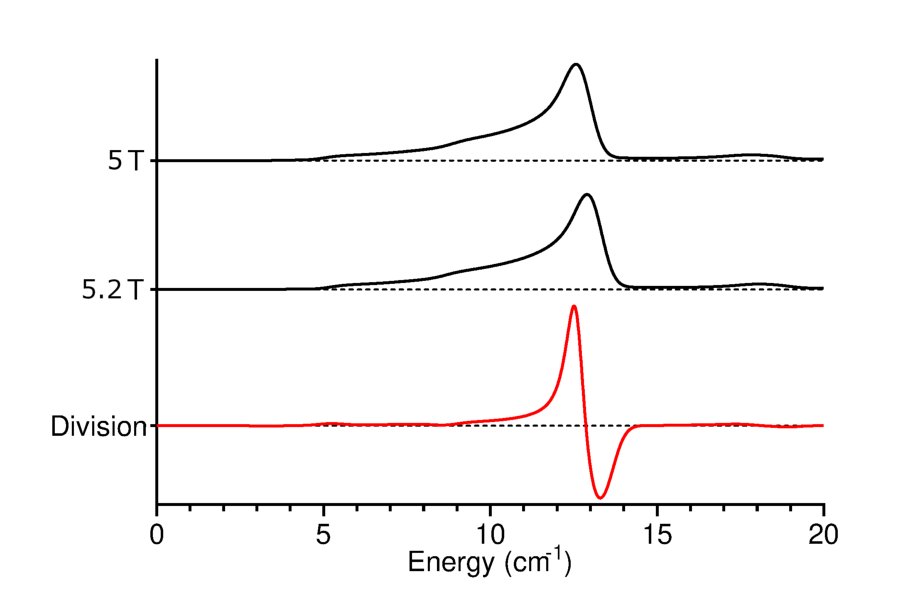
\includegraphics[width=0.8\textwidth]{Kapitel/Ch4-Images/Ch4-ExperimentExplain.eps}
  \caption[FD-FT THz EPR field division of spectra]{Simulated FD-FT THz EPR spectra are shown at $B_0$ and $B_0 - 0.2$~T, 5.2 and 5~T. Shown in red is the spectrum after the division process is performed. The large feature around 15~cm$^{-1}$ corresponds to the feature that is measured in this work. EasySpin calculation used $S=5/2$, $g$-value of [2.05 1.95], D of 6.93~cm$^{-1}$, E of 0, line width 0.8~cm$^{-1}$, and at a temperature of 5~K.}
  \label{ch4-fig:FDS}
\end{figure}

As a test sample, hemin (Sigma-Aldrich) was dissolved in dichlormethane and coated on the SRRs. After evaporation of the solvent, the thickness of the hemin film was determined to be approximately 100~$\mu$m. Hemin contains a high-spin Fe$^\text{III}$ ion ($S = 5/2$), which has a large zero-field splitting. \cite{Nehrkorn15,Johnson66,Marathe73,Lang66} Usually one can observe two EPR features, situated at effective $g$-values of around 6 and 2. \cite{Pilbrow90} In this study, we observed the EPR signal at the effective $g$-value of 6. 

The SRRs were produced on a round quartz substrate which can be rotated in the magnet in order to change the orientation of the the SRR relative to the incident electric field of the THz radiation. The SRR resonator was simulated using Ansys Electromagnetics Suite (Pittsburgh, PA, USA; version 19.1; High Frequency Structure Simulator (HFSS)). Each SRR was individually modeled to obtain the electromagnetic characteristics. Nine SRRs were simulated to establish cross-coupling coefficients using the reciprocity theorem. Due to the SRR mode and geometry, minimal cross coupling was calculated (less than 5\% mutual inductance between elements). 

Two experiments are needed in order to measure the fundamental frequency of the SRR loaded with the sample. The first experiment measures the THz TEM-wave intensity spectrum without the SRR and the second measures the intensity spectrum with the SRR coupled to the THz TEM-wave. The absorbance of the SRRs resonance is then calculated by taking the log of the ratio, such that,
\begin{equation}
  A(\omega) = \text{Log}_{10}\frac{\text{I}_{\text{empty}}(\omega)}{\text{I}_{\text{SRRs}}(\omega)},  
\end{equation}
where $\text{I}_{\text{empty}}(\omega)$, and $\text{I}_{\text{SRRs}}(\omega)$, denotes spectra without and with the SRRs, respectively. 


\begin{figure}[htp]
\centering
  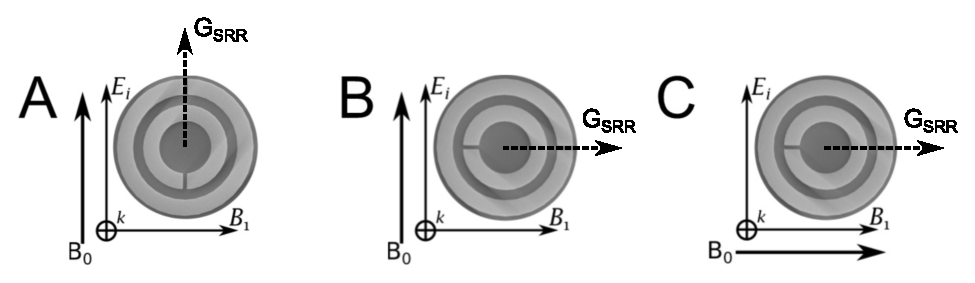
\includegraphics[width=0.8\textwidth]{Kapitel/Ch4-Images/Ch4-BeamPath.eps}
  \caption[THz TEM-wave Orientation Relative to SRR]{Illustrated is the THz TEM-wave orientation relative to the SRR geometry and $\vectu{B}{0}$. Shown is A) $\vectu{B}{1} \perp \vectu{B}{0}$ \& $\vectu{E}{i}||\vectu{G}{SRR}$ B) $\vectu{B}{1} \perp \vectu{B}{0}$ \& $\vectu{E}{i}\perp\vectu{G}{SRR}$ and C) $\vectu{B}{1} || \vectu{B}{0}$ \& $\vectu{E}{i}\perp\vectu{G}{SRR}$.}
  \label{ch4-fig:BeamGEO}
\end{figure}

The path was chosen such that the external magnetic field $\vectu{B}{0}$ was perpendicular to the direction of the THz wave propagation $\vect{k}$, illustrated in Fig.~\ref{ch4-fig:BeamGEO}. Hence, the magnetic ($\vectu{B}{1}$) and electric field ($\vectu{E}{i}$) component of the THz radiation can be chosen parallel or perpendicular to the static magnetic field $\vectu{B}{0}$. This allowed three experiments with different THz electric and magnetic TEM-wave orientations relative to the SRR gaps ($\vectu{G}{SRR}$) and static magnetic field ($\vectu{B}{0}$) to be performed. These experiments are when the propagating $\vectu{B}{1}$ is 

\begin{enumerate}[label=(\Alph*)]
    \item $\vectu{B}{1} \perp \vectu{B}{0}$ \& $\vectu{E}{i}||\vectu{G}{SRR}$: perpendicular to the static magnetic field and the electric field is parallel across the SRR gaps. In this configuration, the SRRs resonance is inactive and only the EPR transition from the incident THz magnetic field can be observed. This configuration is named the ``No Coupling to SRR with EPR Transition'' mode. 
    \item $\vectu{B}{1} \perp \vectu{B}{0}$ \& $\vectu{E}{i}\perp\vectu{G}{SRR}$: perpendicular to the static magnetic field and the electric field is perpendicular across the SRR gaps. In this configuration, both the field from the incident THz magnetic field and coupling to the SRR cause an EPR transition. This configuration  is named the ``Coupling to SRR with EPR Transition'' mode.
    \item $\vectu{B}{1} || \vectu{B}{0}$ \& $\vectu{E}{i}\perp\vectu{G}{SRR}$: parallel to the static magnetic field and the electric field is perpendicular across the SRR gaps. In this configuration, no EPR transition occurs from the THz TEM-wave. However, the SRRs resonance is coupled by the electric field. This configuration is named the ``Coupling to SRR without EPR Transition'' mode.
\end{enumerate}


\section{Theory}
We seek to derive an analytical model of the experiment in order to better understand the complex interactions of the EPR signal with the SRR meta-material. Typically, in antenna design one would choose only magnetic \cite{srrmodel} or electric \cite{Katsarakis04} excitation since magnetic and electric coupling counteract total mutual impedance. Because of this, to our knowledge, the use of both magnetic and electric coupling has not been employed in the literature and for antenna design, only one is necessary to properly describe the coupling of the SRR. \cite{Baena2005,DurnSindreu2012,Bojanic2014,Su2015} We seek to show this is not the case when describing the SRRs in a magnetic resonance experiment. When modeling both the frequency dependence of the SRR and the frequency dependence of the magnetic resonance, both magnetic and electric coupling is needed due to non-zero magnetic field interactions (inductive) and electric field across the gap (capacitive) in the neighborhood of resonance ($\omega_0 - \omega$). This is described in detail and the Mathematica (Wolfram Research, Champaign, Illinois; v.12.1) code can be found in Appendix~B.

Fundamentally, the FD-FT EPR experiment is the measurement of the change in the magnetic susceptibility of the sample as a function of frequency for a given static magnetic field. Therefore we can model the experiment similar to a continuous-wave experiment by defining the permeability as described in Eqn.~\ref{eq-2:permea}. The magnetic susceptibility $\chi(\omega)$ of Eqn.~\ref{eq-2:chi}. For simplicity, the Lorentzian line-shape in the neighborhood of ($\omega_0-\omega$) of Eqn.~\ref{eq-2:chi} was used to mimic the feature at the effective $g$-value of 6. The Lorentzian line-shape reproduces the spectral features well and modeling the true line-shape here does not improve the understanding of the experiment. 

\noindent \paragraph*{Lossless transmission\-/line model with EPR sample.} A free-space lossless transmission\-/line representation includes a series inductance (L$_L$) with the value $\mu_0$ defined as $4 \pi \times 10^{-7}$ [H/m] and shunt capacitance (C$_L$) with the value of $\epsilon_0$ defined as $8.854 \times 10^{-12}$ [F/m]. \cite{ramo1984fields} Therefore, the characteristic impedance of the lossless transmission, defined as
\begin{equation}
    Z_0 = \sqrt{\frac{L_L}{C_L}} = \sqrt{\frac{\mu_0}{\epsilon_0}},
\end{equation}
has a free-space value of 376.7~$\Omega$ and assumes infinitely long propagation. 

As the THz electromagnetic wave interacts with the sample and the magnetic resonance condition is met, a change in the magnetic susceptibility occurs. Since our transmission-line model incorporates a sample, the free-space $\mu_0$ is replaced with $\mu_r(\omega)$ as defined in Eqs.~\ref{eq-2:permea} and \ref{eq-2:chi}. As the static magnetic field is swept, the transimpedance of the wave is modified and the resulting intensity change is recorded.

\noindent \paragraph*{Coupled Resonant Circuit with EPR sample.} Since little mutual coupling occurs between single SRR geometries, it is sufficient to estimate the inductance of a single SRR and model a simplified transmission\-/line coupled system. We can estimate the inductance of the SRR by the classic equation for the inductance of a loop of wire, such that 
\begin{equation}
    L_R(\omega) = \mu_r(\omega) a_r \left(\text{Log}\left[ \frac{8 a_r}{a_w} \right] -2\right),
\end{equation}
where $a_r$ is the effective radius of the loop, and $a_w$ is the radius of the wire. The capacitance of the SRR (C$_R$) can be estimated by the resonance equation $\omega_R^2 L_RC_R=1$, where $\omega_R$ is the resonant frequency of the SRR in radians/s. The resistance is chosen such that the $Q_0$-value matches the measured SRR $Q_0$-value. This is calculated by
\begin{equation}
    Q_0(\omega) = \frac{\omega L_R(\omega)}{R_R} \approx 10.
\end{equation}

\begin{figure*}[htp]
\centering
   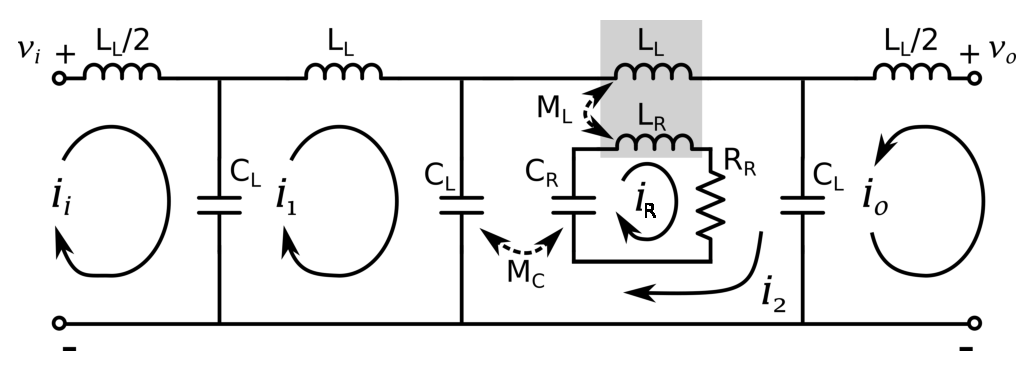
\includegraphics[width=\textwidth]{Kapitel/Ch3-Images/03-CircuitFig.eps}%
  \caption[Transmission\-/line lumped circuit model.]{Transmission\-/line lumped circuit model used to describe the SRR coupling to a plane-wave excitation. Both mutual capacitance ($M_c$) and mutual inductance ($M_L$) are used to describe the circuit. Shown in gray is the region of the circuit where magnetic resonance occurs.}
  \label{ch3-fig:circuit}
\end{figure*}

Using a circuit model of a transmission line with a coupled resonant circuit, illustrated in Fig.~\ref{ch3-fig:circuit}, one can derive the current mesh equations. Such that
\begin{subequations}
\begin{eqnarray}
i(\omega L_L/2 - \frac{1}{\omega C_L}) \text{i}_i +  i\frac{1}{\omega C_L} \text{i}_1 &= v_i  \\
i\frac{1}{\omega C_L} (\text{i}_{i}+\text{i}_2) + i(\omega L_L - \frac{2}{\omega C_L}) \text{i}_{1} + \nonumber \\
 i \omega M_c \text{i}_R &= 0  \\
i\frac{1}{\omega C_L} (\text{i}_{1}-\text{i}_{o}) + i(\omega L_L - \frac{2}{\omega C_L}) \text{i}_{2} + \nonumber \\
i \omega (M_c - M_L) \text{i}_R &= 0  \\
i \frac{1}{\omega C_L} \text{i}_{2} + i(\omega L_L - \frac{2}{\omega C_L}) \text{i}_{o}  &= v_o  \\
i \omega (M_c) \text{i}_{1} + i \omega (M_L - M_c)\text{i}_2 + \qquad \nonumber \\ 
(R_R + i \omega L_R - i\frac{1}{\omega C_R}) \text{i}_R  &= 0
\end{eqnarray}\label{ch3-eq:lineareq}
\end{subequations}

\noindent 
where $v_i$ and $v_o$ is the input and output voltage and $i_i$ and $i_o$ is the input and output mesh currents, respectively, of the transmission-line model, C$_R$ is the capacitance, L$_R$ is the inductance, and R$_R$ is the resistance of the SRR. The mesh currents $i_1$ and $i_2$ are indicated in Fig.~\ref{ch3-fig:circuit} within the transmission line and $i_R$ is the mesh current within the SRR. The mutual inductance ($M_L$) and mutual capacitance ($M_c$) are defined by the coupling coefficients, 
\begin{subequations}
\begin{eqnarray}
    M_c &= k_c \sqrt{C_R C_L}\quad \text{and} \\
    M_L &= k_L \sqrt{L_R L_L}.
\end{eqnarray}
\end{subequations}

The set of linear equations of Eqn.~\ref{ch3-eq:lineareq} are solved for the currents using Wolfram Mathematica.\footnote{It should be noted that L$_R$, L$_L$, $M_L$ are all functions of $\omega$ from the relationship with Eqn.~\ref{eq-2:permea}. This has been removed in the equations for better readability} The relationship of the currents to the voltage is used to find the open-circuit forward transimpedance, where
\begin{equation}
    Z_{21}(\omega) = \frac{v_o}{\text{i}_i} \Biggr\rvert_{\text{i}_o=0} =i \frac{(\omega L_L/2 - \frac{1}{\omega C_L}) \text{i}_o - \frac{1}{\omega C_L} \text{i}_2  }{\text{i}_i} \Biggr\rvert_{\text{i}_o=0}.
\end{equation}

To mimic the FD-FT THz EPR experiment, the open-circuit forward transimpedance $Z_{21}(\omega)$ is evaluated at two EPR resonance frequencies $\omega_0$ from Eqn.~\ref{eq-2:permea} that are 5~GHz apart in order to produce two spectra for the frequency division. These two frequencies in the transmission\-/line model represent the EPR resonance shift that occurs at two static magnetic fields as performed in the FD-FT EPR experiment. The ``resonance shift'' is a parameter that is varied step-wise from 1.0-2.0 in order to shift the spectrum between the energy range of 11-18~cm$^{-1}$. The transmission\-/line model division spectrum is calculated by, 
\begin{equation}
    S(\omega) = \frac{Z_{21}(\omega)\Bigr\rvert_{\omega_0 = \omega_a}}{Z_{21}(\omega)\Bigr\rvert_{\omega_0 = \omega_b}} - 1
\end{equation}
where $S(\omega)$ is the EPR signal and $\omega_a$ and $\omega_b$ are two EPR resonance frequencies representing the resonance shift due to a change in B$_0$. The pair of frequencies $\omega_a$ and $\omega_b$ are stepped across the energy range using a ``resonance shift'' parameter to mimic the change in static magnetic field. In the experiment, and in this model, it is important to note that the SRR resonance energy (frequency) does not change when a static magnetic field is applied. Only the EPR transitions change the system as the magnetic susceptibility $\chi(\omega)$ is stepped through resonance.

\noindent \paragraph*{Strong- and Weak-Coupling Regimes}
When two resonant modes interact, the resulting frequency response greatly depends on the coupling of the two systems. Specifically, the $Q_0$-value of the SRR and the amplitude of the magnetic susceptibility $\chi(\omega)$. Two regimes exist as a continuum: weak-coupling and strong-coupling. 

The weak-coupling regime is characterized as only a perturbation as the EPR resonance passes through the SRR resonance when the static magnetic field is stepped. Weak-coupling interactions results in small shifts of the SRR frequency and $Q_0$-value. If one measures the change in these SRR parameters, a typical EPR experiment would be performed. The measured shift in SRR frequency and $Q_0$-value would correspond to dispersion and absorption signals, respectively. \cite{abragam1961, poole} Weak-coupling regime is desired for EPR experiments using meta-material surfaces.

However, as the concentration of the sample increases (increasing the magnetic susceptibility $\chi(\omega)$) or the $Q_0$-value increases, these systems can exhibit mode-splitting and an anti-crossing feature centered around the frequency where the resonances coincide. This regime, called strong-coupling, is intensified by resonant structures with large filling factors and can be likened to radiation damping. \cite{BloembergenRadDamp, BloomRadDamp, MeiboomRadDamp} One consequence of radiation damping is the second-order effect of the sample changing the current distributions of the resonator as it passes through resonance. Some qualitative understanding of a system with strong-coupling in the context of EPR has led to the understanding of this effect by means of the two-coupled oscillator problem. \cite{SchneiderEPR,BOERO2013133} Herein it is shown that the lumped-circuit transmission\-/line model approximates this interaction. 

\section{Results and Discussion}
The magnitude of the electric and magnetic field profile at the resonance frequency of the SRR is shown in Figs.~\ref{ch3-fig:HFSS}A and ~\ref{ch3-fig:HFSS}B, respectively. The dotted line represents the cut plane plotted to the right. In order to better assess the EPR sensitivity of the SRR with a 100~$\mu$m sample, the THz magnetic field squared is plotted in Fig.~\ref{ch3-fig:HFSS}C along the axis of the SRR. The magnetic field squared is proportional to the EPR signal. In Fig.~\ref{ch3-fig:HFSS}, we plot a dash-dot line at 24~$\mu$m where the area between the quartz substrate surface (0~$\mu$m) and 24~$\mu$m represents 90\% of the EPR signal.

\begin{figure}[htp]
\centering
  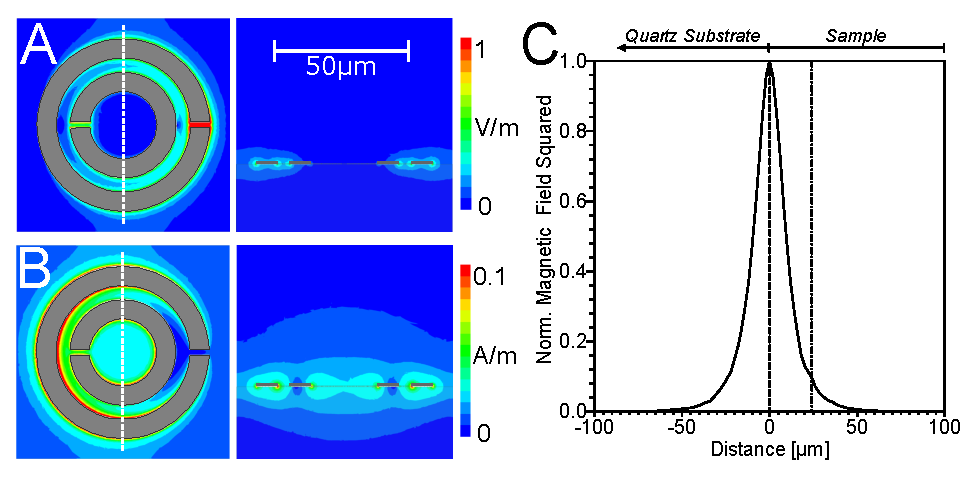
\includegraphics[width=0.9\textwidth]{Kapitel/Ch3-Images/02-AnsoftFields.eps}%
  \caption[Finite-element simulation solutions of SRR geometry.]{Finite-element modeling solutions plotting the magnitude of the THz A) electric and B) magnetic field profile of the SRR. Cut plane is shown as a dotted line. C) Simulated THz magnetic field profile squared (proportional to EPR signal) on the axis of the SRR. The plot starts from -100~$\mu$m into the quartz substrate and  through the SRR until the depth of the sample at 100~$\mu$m. The dash-dot line shows that 90\% of the EPR signal originates from a depth of 24~$\mu$m.}
  \label{ch3-fig:HFSS}
\end{figure}

Shown in Fig.~\ref{ch3-fig:resonator} (dashed line) is the result of the measurement at a temperature of 2~K and in the absence of an external static magnetic field. This absorbance was then normalized to compare to simulations. Simulations are shown in Fig.~\ref{ch3-fig:resonator} as a solid line. The absorption feature is associated with the lowest-order resonance mode of the SRRs. \cite{Katsarakis04} Without the sample, at an energy of 14.47 cm$^{-1}$, a pronounced absorbance with full width at half maximum (FWHM) of 1.45 cm$^{-1}$ was observed. After the thin film of hemin is placed on top of the SRRs, a shift of the absorbance to lower energy of 13.97 cm$^{-1}$, accompanied by slight narrowing of the FWHM to 0.87 cm$^{-1}$, was observed. The absorptive feature could be identified in the intensity spectrum (not shown). Using the FWHM, $Q_0$-values of 10 and 17 were measured for both the SRR without sample and the SRR with hemin sample, respectively. Simulations show the SRRs resonance at 13.76 cm$^{-1}$ for SRRs with sample. The deviation of the simulation from the experiment is only 1.5\%. The very good agreement is due to the high quality of the manufacturing of the SRRs. The $Q_0$-value of the simulated SRR is 42. The discrepancy is due to the unknown loss tangent of the hemin sample at THz frequencies.


\begin{figure}[htp]\centering
  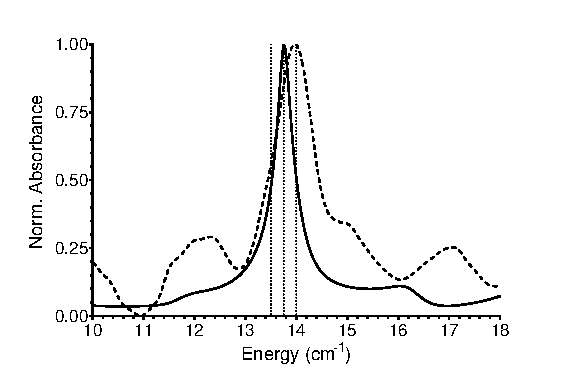
\includegraphics{Kapitel/Ch3-Images/03-SRR_Profile.eps}%
  \caption[Simulated and measured SRR resonance.]{Resonance condition of the SRR meta-material with 100~$\mu$m sample calculated using HFSS (solid) and measured (dashed) shown by plotting the normalized absorbance.}
  \label{ch3-fig:resonator}
\end{figure}

\begin{figure}[htbp]\centering
  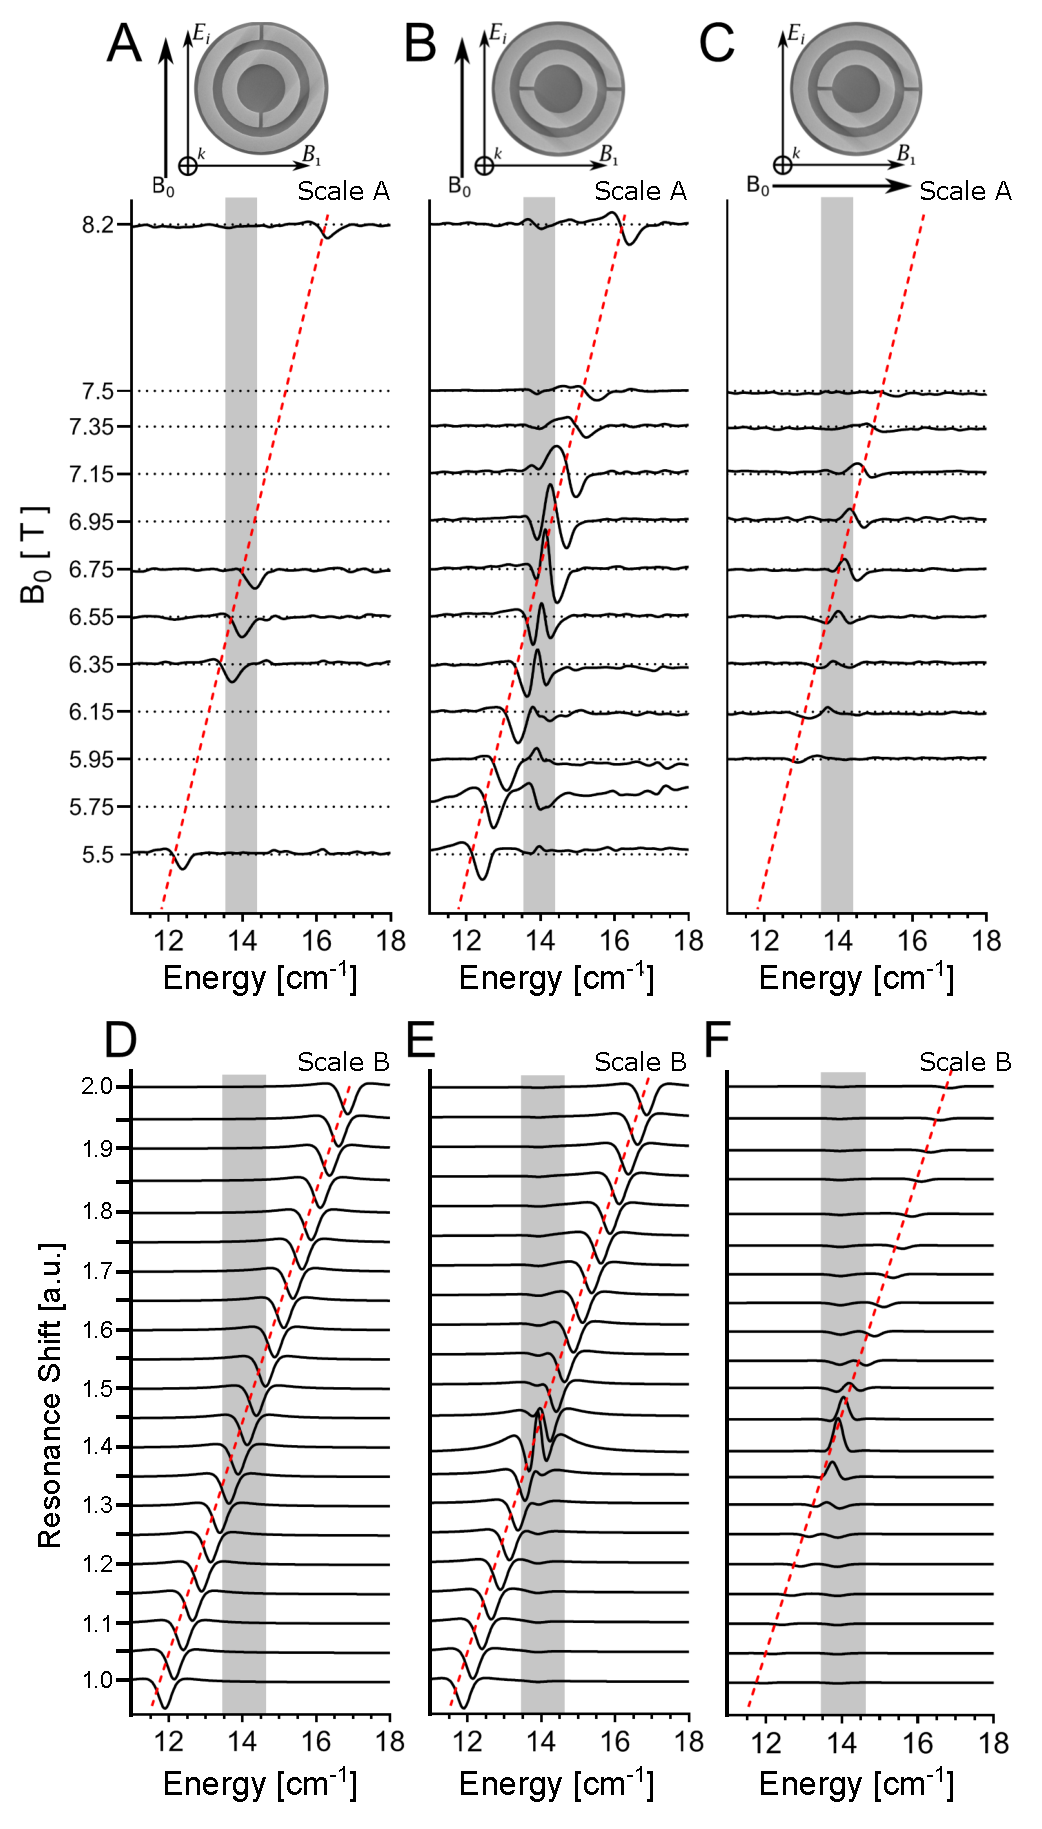
\includegraphics[width=0.7\textwidth]{Kapitel/Ch3-Images/HugeData.eps}%
  \caption[FD-FT EPR Data and Lumped-Circuit Model with SRRs]{Measured data and lumped-circuit model EPR signal interacting with the SRRs. The red dotted line indicates the calculated transition energy. The gray shaded area indicates the bandwidth of the SRRs with the sample. The SRRs are depicted by a single SRR. The direction of the external magnetic field $\vectu{B}{0}$is shown compared to the THz radiation travelling wave normal to the SRRs, i.e the $\vect{k}$ vector goes into the paper, with electric $\vect{E}_i$ and magnetic $\vect{B}_1$ components indicated. The measurements in the three configurations are: A) No Coupling to SRR with EPR Transition, B) Coupling to SRR with EPR Transition, and C) Coupling to SRR without EPR Transition. The series is repeated using the lumped-circuit model and displayed in D-F.\label{ch3-fig:datacompare}}
\end{figure}

The EPR transition will only be observed for the magnetic field component of the THz radiation $\vectu{B}{1}$ perpendicular to the external magnetic field $\vectu{B}{0}$ ($\vectu{B}{1} \perp \vectu{B}{0}$). \cite{Nehrkorn15_PRL} Additionally, the resonance of the SRRs only couple to the THz radiation if the electric field is parallel to the gap of the rings of the SRRs ($\vectu{E}{i}\perp\vectu{G}{SRR}$). \cite{Katsarakis04} The results of a series of FD-FT EPR experiments can be found in Fig.~\ref{ch3-fig:datacompare}A-C and each measurement is described below. The spectra of Fig.~\ref{ch3-fig:datacompare}A-C are on the same scale (indicated as Scale A).

\noindent \paragraph*{No Coupling to SRR with EPR Transition.} In this configuration we could observe the feature at the effective $g$-value of 6 of high-spin Fe with almost unchanged intensity over the measured field and frequency range, shown in Fig.~\ref{ch3-fig:datacompare}A. This data confirms the SRRs resonance was inactive since only the EPR transition was observed. 

\noindent \paragraph*{Coupling to SSR with EPR Transition.} Measured data, shown in Fig.~\ref{ch3-fig:datacompare}B, exhibited an increase in the intensity of the EPR signal of hemin in the frequency range where the EPR line and the SRRs resonance overlap. Over this region a complex interaction occurs where real and imaginary parts of the magnetic susceptibility $\chi(\omega)$ mix with the frequency dependent effective $\mu(\omega)$ and $\epsilon(\omega)$ of the SRR.

\noindent \paragraph*{Coupling to SSR without EPR Transition.} In this experiment, $\vectu{B}{1}$ is parallel to $\vectu{B}{0}$ and, as such, EPR transitions should not be observed. However, in the region where the EPR line overlaps with the resonance of the SRRs a feature was observed, data shown in Fig.~\ref{ch3-fig:datacompare}C. This can be rationalized by a magnetic field component $\vectu{B}{1}\perp\vectu{B}{0}$ that arises from the SRR geometry since $\vectu{E}{i}$ is perpendicular to the SRR gaps ($\vectu{G}{SRR}$). Hence, the observed EPR line was a direct proof that an additional THz magnetic field was generated by the SRRs resonance. This configuration demonstrates the use SRRs in resonance with THz radiation for resonant EPR detection at a single frequency. 

\noindent \paragraph*{Transmission\-/line model: Results.} Parameters to duplicate the FD-FT THz EPR experiments using the lumped-circuit transmission\-/line model of Fig.~\ref{ch3-fig:circuit} are shown in Table~\ref{ch3-table:lumpedparameters}. The inductance L$_r(\omega)$, capacitance C$_r$, and resistance R$_r$ needed to describe the SRR were found by calculating the inductance of a small loop (diameter 20~nm and wire thickness $19 \times 10^{-12}$m and setting the capacitance to resonant at 13.9~cm$^{-1}$. The resistance chosen gives a $Q_0$-value of 10. The phenomenologically chosen EPR characteristics T$_1$, T$_2$, and $\gamma$ give a Lorentzian line of suitable width to approximate the experimentally observed feature at the effective $g$-value of 6 as measured in Fig.~\ref{ch3-fig:datacompare}A. 

\begin{table}[hbtp]
\centering
\caption{Parameters used for the lumped-circuit model characterization.}
\begin{tabular}{l|c}
\multicolumn{1}{l|}{Param.} & \multicolumn{1}{c}{Values} \\ \hline \hline
\multicolumn{1}{l|}{$L_r$} & \multicolumn{1}{c}{$29.76\times 10^{-15}$~H} \\
\rowcolor[rgb]{0.937,0.937,0.937}  
\multicolumn{1}{l|}{$C_r$} & \multicolumn{1}{c}{$4.89\times 10^{-12} $~F} \\
\multicolumn{1}{l|}{$R_r$} & \multicolumn{1}{c}{$0.008~\Omega$} \\
\rowcolor[rgb]{0.937,0.937,0.937}  
\multicolumn{1}{l|}{T$_1$} & \multicolumn{1}{c}{$4\times 10^{-9}$~s} \\
\multicolumn{1}{l|}{T$_2$} & \multicolumn{1}{c}{$0.1\times 10^{-9}$~s} \\
\rowcolor[rgb]{0.937,0.937,0.937}  
\multicolumn{1}{l|}{$\gamma$} & \multicolumn{1}{c}{$2.8$~MHz/G}
\end{tabular}\label{ch3-table:lumpedparameters}
\end{table}

The integral of the magnetic susceptibility $\chi(\omega)$ of Eqn.~\ref{eq-2:chi} was normalized and the parameters $g_f$ and $g_r$ were used for scaling. The parameters encompass the filling factor $\eta$ and number of spins for the free-space and resonant signals, $g_f$ and $g_r$, respectively. From the right-hand side of Eqn.~\ref{eq-2:permea}, the substitution
\begin{equation}
    \eta \chi(\omega) =
    \begin{cases}
      g_f \hat{\chi}(\omega), & \text{for free-space}\ L_L(\omega) \\
      g_r \hat{\chi}(\omega), & \text{for resonator}\ L_R(\omega)
    \end{cases}
\end{equation}\label{etagfgr}
where $\hat{\chi}(\omega)$ is the normalized magnetic susceptibility. Therefore, adjusting  $g_f$ and $g_r$ affects the EPR signal intensity by scaling $\mu_r(\omega)$ in L$_L(\omega)$ and L$_r(\omega)$, respectively, in the lumped-circuit transmission\-/line model. The parameters $g_f$ and $g_r$ can be visualized in the illustration of Fig.~\ref{ch3-fig:effetachi}. The parameter $g_f$ represents the whole sample that is excited by the THz plane-wave travelling through the sample, illustrated as the blue hatch in Fig.~\ref{ch3-fig:effetachi}A. The parameter $g_r$ represents only the sample that is excited by the SRRs, illustrated as the blue hatch in Fig.~\ref{ch3-fig:effetachi}B. When both the EPR transitions and SRR are coupled ($\vectu{B}{1}\perp\vectu{B}{0}$ and $\vectu{E}{i}\perp\vectu{G}{SRR}$) the linear combination of Figs.~\ref{ch3-fig:effetachi}A and \ref{ch3-fig:effetachi}B is excited. The spectra of Figs.~\ref{ch3-fig:datacompare}D-F use the same $g_f$ and $g_r$ parameters and, therefore, are on the same scale (indicated as Scale B). The parameters used to characterize the coupling and EPR signal for the lumped-circuit model are found in Table~\ref{ch3-table:parameters}.

\begin{figure}[htbp]\centering
  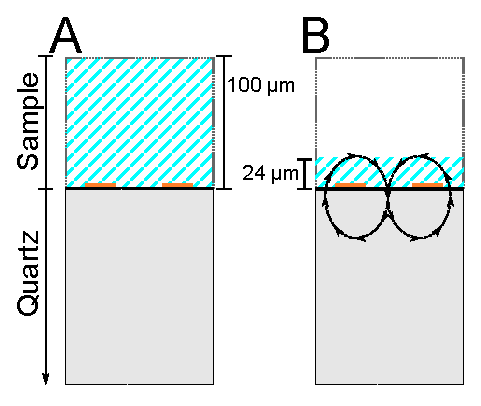
\includegraphics{Kapitel/Ch3-Images/Ch4-SampleVisualization.eps}%
  \caption[Illustration of the excited sample volumes.]{An illustration showing the effective volume for A) the experiment without SRRs coupling and B) the experiment with only SRRs coupling. Here the hatched blue area is the volume of spins and the gray area is the quartz substrate. The THz magnetic field vectors (dashed arrows) are illustrated for the SRR geometry (orange).
  \label{ch3-fig:effetachi}}
\end{figure}

In the calculation, coupling was adjusted using the inductive $k_L$ and capacitive $k_c$ coupling constants and fit to the data of Fig.~\ref{ch3-fig:datacompare}B. It is noted that the coupling constants are not unique. Nevertheless, one interesting outcome of this model is the ratio of the amplitude parameters $g_f$ and $g_r$. A factor of 4.7 is realized for the apparent intensity of the EPR spins in the 24~$\mu$m region. This result is consistent with the THz magnetic field squared profile of Fig.~\ref{ch3-fig:HFSS}C showing a factor of 4.2 for the sample to active-region ratio compared to Fig.~\ref{ch3-fig:HFSS}B. This is reproduced in Figs.~\ref{ch3-fig:HFSS}D and ~\ref{ch3-fig:HFSS}F.

\begin{table}[htp]
\centering
\caption{Parameters used for the EPR characterization using the lumped-circuit model. The following configurations of A) $\vectu{B}{1}\!\perp\!\vectu{B}{0}$ \& $\vectu{E}{i}||\vectu{G}{SRR}$, B) $\vectu{B}{1}\!\perp\!\vectu{B}{0}$ \& $\vectu{E}{i}\!\perp\!\vectu{G}{SRR}$, and C) $\vectu{B}{1}||\vectu{B}{0}$ \& $\vectu{E}{i}\!\perp\!\vectu{G}{SRR}$ are shown. }
\begin{tabular}{ll}
%\multicolumn{1}{r}{}&{$\vectu{B}{1}\!\perp\!\vectu{B}{0}$ \& $\vectu{E}{i}||\vectu{G}{SRR}$} \\
\multicolumn{1}{r}{\textbf{{\Large A.}}}&{} \\
\multicolumn{1}{l|}{} & \multicolumn{1}{c}{Values} \\ \hline \hline
\multicolumn{1}{l|}{$g_f$} & \multicolumn{1}{c}{$10\times 10^{-6}$} \\
\rowcolor[rgb]{0.937,0.937,0.937}  
\multicolumn{1}{l|}{$g_r$} & \multicolumn{1}{c}{$47\times 10^{-6}$} \\
\multicolumn{1}{l|}{$k_c$} & \multicolumn{1}{c}{0} \\
\rowcolor[rgb]{0.937,0.937,0.937}  
\multicolumn{1}{l|}{$k_L$} & \multicolumn{1}{c}{0.065}\\
\end{tabular}\hspace{1em}
\begin{tabular}{ll}
%\multicolumn{1}{r}{}&{$\vectu{B}{1}\!\perp\!\vectu{B}{0}$ \& $\vectu{E}{i}\!\perp\!\vectu{G}{SRR}$} \\
\multicolumn{1}{r}{\textbf{{\Large B.}}}&{} \\
\multicolumn{1}{l|}{} & \multicolumn{1}{c}{Values} \\ \hline\hline
\multicolumn{1}{l|}{$g_f$} & \multicolumn{1}{c}{$10\times 10^{-6}$} \\
\rowcolor[rgb]{0.937,0.937,0.937}  
\multicolumn{1}{l|}{$g_r$} & \multicolumn{1}{c}{$47\times 10^{-6}$} \\
\multicolumn{1}{l|}{$k_c$} & \multicolumn{1}{c}{0.255} \\
\rowcolor[rgb]{0.937,0.937,0.937}  
\multicolumn{1}{l|}{$k_L$} & \multicolumn{1}{c}{0.065}
\end{tabular}\hspace{1em}
\begin{tabular}{ll}
%\multicolumn{1}{r}{}&{$\vectu{B}{1}||\vectu{B}{0}$ \& $\vectu{E}{i}\!\perp\!\vectu{G}{SRR}$} \\
\multicolumn{1}{r}{\textbf{{\Large C.}}}&{} \\
\multicolumn{1}{l|}{} & \multicolumn{1}{c}{Values} \\ \hline\hline
\multicolumn{1}{l|}{$g_f$} & \multicolumn{1}{c}{0} \\
\rowcolor[rgb]{0.937,0.937,0.937}  
\multicolumn{1}{l|}{$g_r$} & \multicolumn{1}{c}{$47\times 10^{-6}$} \\
\multicolumn{1}{l|}{$k_c$} & \multicolumn{1}{c}{0.255} \\
\rowcolor[rgb]{0.937,0.937,0.937}  
\multicolumn{1}{l|}{$k_L$} & \multicolumn{1}{c}{0.065} 
\end{tabular}\label{ch3-table:parameters}
\end{table}

Using the transmission\-/line model, the ``EPR Transition without SRR Coupling'' mode is realized by setting the coupling constant $k_c$ to zero, illustrated in Fig.~\ref{ch3-fig:datacompare}D and with parameters reproduced in Table~\ref{ch3-table:parameters}A. The magnetic coupling constant $k_L$ is not set to zero because there is some component of the THz magnetic field that generates a small current on the SRR as shown by the simulations of the surface currents in Fig.~\ref{ch3-fig:surfacecurrent}. The scattering magnetic field from the surface currents generated by magnetic coupling does not perturb the EPR transitions from the THz TEM-wave. The transmission\-/line model results of the ``EPR Transition without SRR Coupling'' mode are shown in Fig.~\ref{ch3-fig:datacompare}D.

\begin{figure}[htbp]\centering
  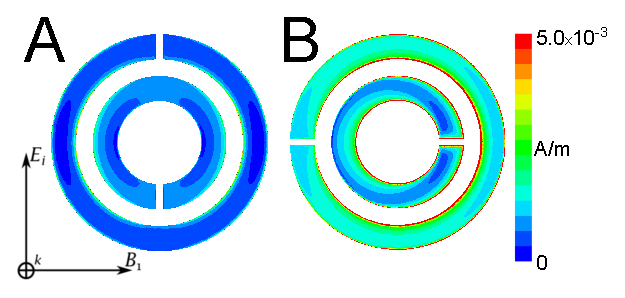
\includegraphics{Kapitel/Ch3-Images/SurfaceCurrent-THz.eps}%
  \caption[Simulation of the surface currents for SRR coupling.]{Simulation of the surface currents for SRR coupling. The plane wave used in order to excite both profiles is shown on the left. A) When the SRR is not coupled to the THz TEM-wave ($\vectu{E}{i}||\vectu{G}{SRR}$) there exists surface currents from inductive coupling, $k_L$. B) When the SRR is coupled to the THz TEM-wave ($\vectu{E}{i}\perp\vectu{G}{SRR}$) surface currents are generated by capacitive coupling, $k_c$.} \label{ch3-fig:surfacecurrent}
\end{figure}


In the ``Coupling to SRR with EPR Transition'' mode, the EPR transitions occur ($g_f$ is non-zero) and the SRRs are coupled. Using the transmission\-/line model, the response of the coupled resonance shown in Fig.~\ref{ch3-fig:datacompare}B is duplicated. Data is plotted in Fig.~\ref{ch3-fig:datacompare}E and with parameters reproduced in Table~\ref{ch3-table:parameters}B. The change in spectral shape shown in Figs.~\ref{ch3-fig:datacompare}B and \ref{ch3-fig:datacompare}E can be interpreted as a phase shift between the EPR transition and the frequency dependent effective $\mu(\omega)$ and $\epsilon(\omega)$ of the SRR. The phase shift is directly related to the capacitive (electric) and inductive (magnetic) coupling $k_c$ and $k_L$, respectively. The spectral shape cannot be reproduced without the small magnetic coupling $k_L$. The magnetic coupling is enhanced at resonance and both electric and magnetic coupling was required to fit the model to the experiment.

In the ``Coupling to SRR without EPR Transition'' mode, the EPR transitions do not occur ($g_f$ is zero), but the SRRs are coupled to the THz TEM-wave. The effect of the coupled resonance is duplicated in the calculated data using the lumped-circuit impedance, shown in Fig.~\ref{ch3-fig:datacompare}B and with parameters reproduced in Table~\ref{ch3-table:parameters}C. 

At the SRR resonance, a magnetic resonance feature around 14~cm$^{-1}$ can be seen that does not shift with magnetic field, shown clearly in Fig.~\ref{ch3-fig:datacompare}B at a static magnetic field of 8.2~T. This feature is also shown in calculated data in Figs.~\ref{ch3-fig:datacompare}E and ~\ref{ch3-fig:datacompare}F. This is an interesting feature that, at the time, was thought to be noise, since any EPR transition should follow the linear step of the magnetic field. However, the enhancement provided by the SRRs results in an increase in the sensitivity. This enhancement of the ``tails'' of the EPR line are detectable even at the edge of the neighborhood of resonance ($\omega_0-\omega$). With the transmission\-/line model, we show this effect can be enhanced by approaching the strong-coupling domain.

\noindent \paragraph*{Transmission\-/line model: Weak- and Strong Regime.} From the transmission\-/line model, we can say that we are in a weak-coupling regime, illustrated in Fig.~\ref{ch3-fig:strong-weak}. Here the solid line represents the frequency shift using the parameters in Table.~\ref{ch3-table:parameters}C. A weak-coupling frequency perturbation is apparent at a simulated ``resonance shift'' of 1.4 (black dotted). The perturbation is compared to a constant SRR frequency of 420~GHz, represented as a dashed line. As the concentration increases, the magnetic susceptibility $\chi(\omega)$ increases and a non-linear effect occurs between the EPR transition and the resonant frequency of the SRR. When this occurs, the system approaches the strong-coupling regime. This is characterized by two resonances ($\CIRCLE$ and $\blacksquare$) interacting and creating an anti-crossing profile. A third resonance, denoted by the symbol $\hexagon$ occurs as the linear shift crossing displaying the onset of strong-coupling. In Fig.~\ref{ch3-fig:strong-weak}, $g_f$ was set to zero and $g_r$ was increased 100 fold to create the strong-coupling regime compared to the model used to describe the experiment of Fig.~\ref{ch3-fig:datacompare}F and Table~\ref{ch3-table:parameters}C. In practice, the increased in $g_r$ by 100 fold is equivalent to increasing the sample concentration by 100.

\begin{figure}[htp]\centering
  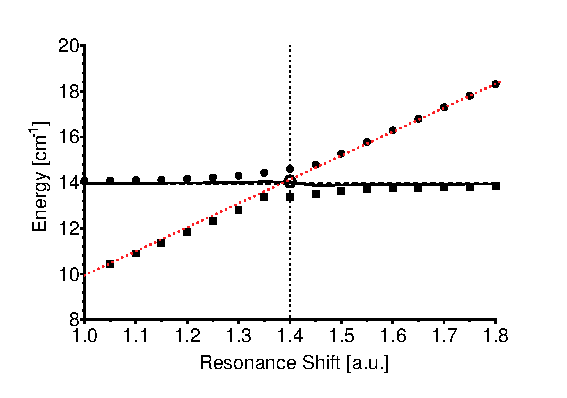
\includegraphics{Kapitel/Ch3-Images/08-RadiationDampening.eps}%
  \caption[Calculated weak- and strong-coupling regime using the analytical model.]{Using the lumped-circuit transmission\-/line model of Fig.~\ref{ch3-fig:circuit}, a weak- and strong-coupling plot can be obtained. Shown along side is a constant microwave energy (approximately 14~cm$^{-1}$; dashed). The crossover point is illustrated as a dotted line and represents a SRR resonance at 1.4. The weak-coupling regime is produced by the parameters in Table~\ref{ch3-table:parameters}C and is plotted as a black solid line. The symbols $\hexagon$, $\CIRCLE$, and $\blacksquare$ represent the frequencies in the strong-coupling regime, while the red dashed line represents the linear shift of the EPR signal as the static magnetic field is shifted.}\label{ch3-fig:strong-weak}
\end{figure}

\section{Conclusions and Outlook}
We have simulated and experimentally verified SRRs structures for use at very high-frequency EPR of thin films. The very good agreement between finite-element modeling simulations and the fabricated SRRs allowed us to investigate the interaction of the SRRs with the EPR line of a high-spin system. Our experiments revealed an increased EPR intensity by a factor of approximately 4 for an effective sample depth of 24~$\mu$m when the SRRs are employed as a surface resonator. Results were further confirmed using an lumped-circuit lossless transmission\-/line model which incorporates both magnetic and electric field coupling. The lumped-circuit model provides a unique way to study the interaction of spin-ensembles with meta-materials as the EPR transitions are swept through resonance. From first-principles, the EPR transitions have been included in lumped-circuit model permeability $\chi(\omega)$ which is then ``detected'' by the change in the transimpedance of the coupled system.

Unlike meta-material literature for antennas, in this work, both magnetic and electric field coupling was required to match the experimental data. When designing an meta-material based antenna, the inductive coupling and capacitive coupling would cancel each other out over a finite frequency range and provide only a bulk frequency-dependant effective $\mu(\omega)$ and $\epsilon(\omega)$. However, when the SRR is used as a surface resonator for EPR and is covered with a sample, the inductance L$_L(\omega)$ and mutual inductance $M_L(\omega)$ become a function of the EPR signal. This implies they are no longer just parameters for coupling. Conversely, the electric field mutual capacitance $M_C$ does not vary with EPR magnetic resonance. This shift in inductive coupling in the neighborhood of EPR resonance contributes considerable to the shape of the measured signal.

The lumped-circuit transmission\-/line model gives us a good representation of the meta-material enhanced FD-FT THz EPR experiment in order to optimize the experiment for the study of diluted samples in thin films. With the SRRs described here, one could perform multi-frequency high-field EPR experiments. \cite{KRZYSTEK2006,Telser2014} Such multi-frequency high-field EPR experiments would require a number of meta-material resonant discs to be fabricated with resonances at multiple frequencies. A series of SRRs could be used to obtain broadband information allowing for the study of diluted protein samples.

The use of meta-materials and further understanding presented here provides a framework to design more complicated meta-material unit structures. By changing the geometry of the unit structure from a SRR, the use of meta-materials can be tuned for EPR spectroscopy. \cite{ZhangMetasurfaces}


{\renewcommand{\bibsection}{\clearpage\section*{\bibname}\markboth{\bibname}{\bibname}}
\renewcommand{\bibname}{CHAPTER 4. REFERENCES}
\bibliographystyle{elsarticle-num}
\bibliography{Kapitel/Ch4-References}
}